\section{Nuclei mass measurements with regard to nuclear force theory}
The mention of binding energy and results was previously stated.
Another analysis we could do on nucleon binding energies is investigating the magic numbers of nucleons.
The idea is that there is a section on the nucleon landscape that is stable.
Before the discovery of the standard 2, 8, 30, 28, 50, 82, 126 magic numbers, higher values of 184, 258, 350, and 462 are thought to exist. 
The existence of these number are theoretical and are calculated based on the Binomial coefficient.

\subsection{Nucleon pairing energy}
Besides the standard investigations, we can also investigate the neutron pairing energy of finite nuclei.
We can study a range of odd and even pairs of N/Z numbers; to investigate the strong nuclear force \cite{fred_neutron_2019}.
So far, the idea is that the (N)even-(Z)even nucleus (although energy depends on factors such as the kind of particles and state it is occupied) we known for a fact that odd(N)- odd(A) nucleus is 1/2 to 2/3 times smaller, this is when they are given in the same shell and the mass numbers A are very close to one another.
This strange character is due to the nucleon-nucleon potential resulting from the strong force. \cite{jensen_elementary_1955}

There is a model known as the liquid drop model, which underpredicts the binding energy of magic nuclei, magic nuclei referrer to nuclei where N or Z are a magic number, for the stable atoms these are 2, 8, 20, 28, 50, 82 and 126.
The neutron/proton separation energy peaks if N(Z) equals a magic number; on \cref{fig:MSaNFTzigzag}, we see this as the last point before the significant drop.
There is a more stable isotope if Z is a magic number and a more stable isotone if N is a magic number.
If either N or Z or both are magic numbers, then the energies of the excited state will be much higher than the ground state.
Another discovery is that elements with Z equal to a magic number have a more prominent natural abundance than nearby elements. \cite{kumawat_description_2018}

\begin{figure}[H]
    \centering
    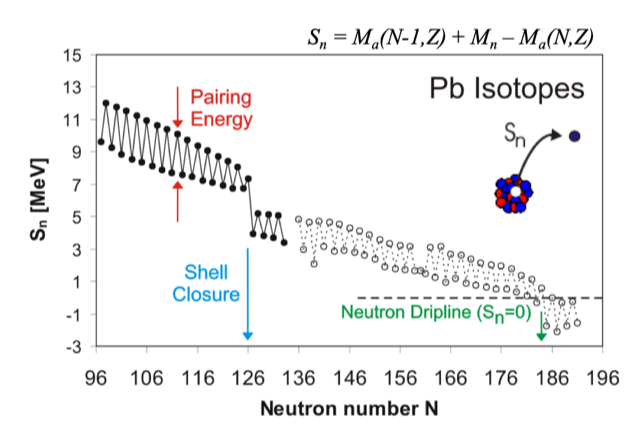
\includegraphics[width=.5\textwidth]{images/MSaNFT_zigzag.png}
    \caption{Neutron binding energy for lead isotopes. In blue a shell closure is highlighted at 126N. The sharp oscillations in energy highlight neutron pairing energies \cite{noauthor_nuclear_nodate}.}\label{fig:MSaNFTzigzag}
\end{figure}

\subsection{Liquid drop model and the investigation of magic numbers}
The magic number can further be explained by the shell closure model of the nucleus.
This is done by considering each nucleon to be moving in some potential and classifying the energy level in terms of quantum numbers n l j, like how the wavefunction of individual electrons are classified in atomic physics.
The energy eigenvalues depend on the principal quantum number, n, orbital angular momentum.
The energy level comes in shells, with a large gap just above each shell. \cite{smolanczuk_particle}

\subsection{Nucleon driplines}
In particle physics, we often use the idea of drip lines to categorize our particles.
We have a one or two-particle drip line, which is a result of the idea that odd and even nucleon numbers, as we know, it has a significant effect on binding energy.
We will be looking at one particle drip line for an odd(Z) or odd(N) nuclei.
Experimentally, we determined the one and two neutron drip lines up to neon. [??tobedone??]